\documentclass{standalone}

% graphics
\usepackage{tikz}
\usepackage{pgfplots}
\usepackage{siunitx}

\begin{document}

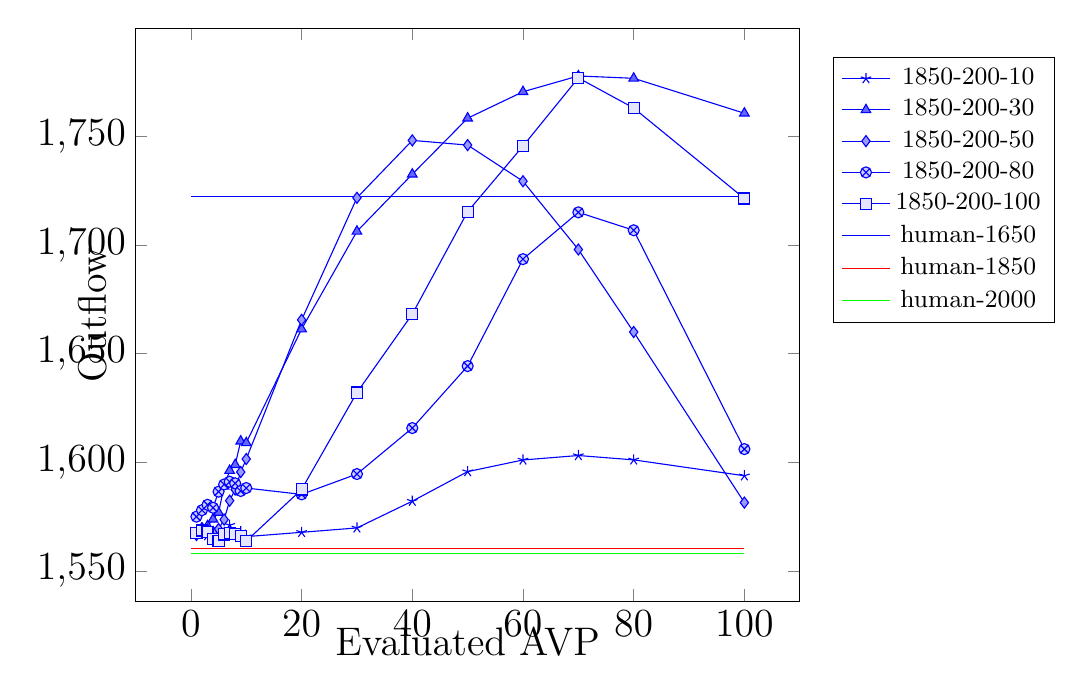
\begin{tikzpicture}[scale=1]
  \pgfplotsset{
      scale only axis,
      every x tick label/.append style={font=\Large},
      every y tick label/.append style={font=\Large},
	legend style={at={(1.05,0.95)},anchor=north west}
  }

\pgfplotscreateplotcyclelist{mycolorlist}{%
	blue,every mark/.append style={fill=blue!80}, mark=star, error bars/.cd, y dir=both, y explicit\\%
	blue,every mark/.append style={fill=blue!60}, mark=triangle*, error bars/.cd, y dir=both, y explicit\\%
	blue,every mark/.append style={fill=blue!40}, mark=diamond*, error bars/.cd, y dir=both, y explicit\\%
	blue,every mark/.append style={fill=blue!20}, mark=otimes*, error bars/.cd, y dir=both, y explicit\\%
	blue,every mark/.append style={fill=blue!10}, mark=square*, error bars/.cd, y dir=both, y explicit\\%
	red,densely dashed,every mark/.append style={solid,fill=red!80}, mark=star, error bars/.cd, y dir=both, y explicit\\%
	red,densely dashed,every mark/.append style={solid,fill=red!60},mark=triangle*, error bars/.cd, y dir=both, y explicit\\%
	red,densely dashed,every mark/.append style={solid,fill=red!40},mark=diamond*, error bars/.cd, y dir=both, y explicit\\%
	red,densely dashed,every mark/.append style={solid,fill=red!20}, mark=otimes*, error bars/.cd, y dir=both, y explicit\\%
	red,densely dashed,every mark/.append style={solid,fill=red!10}, mark=square*, error bars/.cd, y dir=both, y explicit\\%
	green!40!black, dashed,every mark/.append style={solid,fill=green!80}, mark=star, error bars/.cd, y dir=both, y explicit\\%
	green!40!black, dashed,every mark/.append style={solid,fill=green!60},mark=triangle*, error bars/.cd, y dir=both, y explicit\\%
	green!40!black, dashed,every mark/.append style={solid,fill=green!40},mark=diamond*, error bars/.cd, y dir=both, y explicit\\%
	green!40!black, dashed,every mark/.append style={solid,fill=green!20},mark=otimes*, error bars/.cd, y dir=both, y explicit\\%
	green!40!black, dashed,every mark/.append style={solid,fill=green!10},mark=square*, error bars/.cd, y dir=both, y explicit\\%
	black, dashed,every mark/.append style={solid,fill=green!80}, mark=star, error bars/.cd, y dir=both, y explicit\\%
	black, dashed,every mark/.append style={solid,fill=green!60},mark=triangle*, error bars/.cd, y dir=both, y explicit\\%
	black, dashed,every mark/.append style={solid,fill=green!40},mark=diamond*, error bars/.cd, y dir=both, y explicit\\%
	black, dashed,every mark/.append style={solid,fill=green!20},mark=otimes*, error bars/.cd, y dir=both, y explicit\\%
	black, dashed,every mark/.append style={solid,fill=green!10},mark=square*, error bars/.cd, y dir=both, y explicit\\%
	}


\begin{axis}[
    legend style={font=\small},
	ylabel={\Large Outflow},
	x label style={at={(axis description cs:0.5,-0.03)},anchor=north},
	y label style={at={(axis description cs:-0.030,0.5)}, anchor=south},
	xlabel={\Large Evaluated AVP},
	cycle list name=mycolorlist
]

\addplot table [x=a, y=b] {
a	 b	 c
1	1567.48	20.0
2	1569.13	15.5
3	1566.22	21.17
4	1564.31	18.49
5	1565.46	21.49
6	1567.87	21.73
7	1571.08	24.53
8	1567.33	21.86
9	1568.05	19.95
10	1565.82	19.36
20	1567.8	21.88
30	1569.82	21.43
40	1582.13	27.96
50	1595.74	24.05
60	1601.1	27.05
70	1603.15	23.34
80	1601.14	21.96
100	1593.83	25.51
};
\label{1850-200-10}

\addplot table [x=a, y=b] {
a	 b	 c
1	1566.32	23.76
2	1569.46	26.48
3	1570.75	29.4
4	1573.81	29.34
5	1576.94	31.49
6	1588.93	34.98
7	1596.2	38.93
8	1598.9	35.64
9	1609.74	41.99
10	1608.98	36.2
20	1661.36	52.72
30	1706.33	59.0
40	1732.61	50.25
50	1758.42	49.65
60	1770.59	48.19
70	1777.86	40.57
80	1776.78	37.07
100	1760.69	34.8
};
\label{1850-200-30}

\addplot table [x=a, y=b] {
a	 b	 c
1	1566.58	20.21
2	1569.71	16.77
3	1568.99	21.58
4	1567.98	20.59
5	1569.31	22.36
6	1573.67	23.79
7	1582.34	27.72
8	1587.49	33.19
9	1595.56	28.19
10	1601.53	33.5
20	1665.58	41.0
30	1721.77	46.37
40	1748.2	48.27
50	1746.04	32.63
60	1729.4	29.12
70	1697.98	30.49
80	1660.0	26.93
100	1581.48	34.21
};
\label{1850-200-50}

\addplot table [x=a, y=b] {
a	 b	 c
1	1575.0	22.11
2	1577.99	21.35
3	1580.47	26.22
4	1579.1	25.62
5	1586.52	25.65
6	1589.83	30.78
7	1591.09	27.9
8	1590.34	28.33
9	1586.81	31.37
10	1588.18	32.12
20	1585.26	37.79
30	1594.62	40.5
40	1615.79	43.2
50	1644.3	54.01
60	1693.55	48.28
70	1715.08	45.51
80	1706.83	36.75
100	1606.1	29.4
};
\label{1850-200-80}

\addplot table [x=a, y=b] {
a	 b	 c
1	1567.48	20.24
2	1568.63	19.29
3	1567.76	23.74
4	1564.78	18.61
5	1563.95	25.09
6	1566.83	24.58
7	1567.62	23.19
8	1567.19	21.82
9	1566.04	21.78
10	1563.77	21.96
20	1587.53	31.58
30	1632.13	33.74
40	1668.24	42.96
50	1715.4	49.85
60	1745.6	51.61
70	1776.96	40.9
80	1763.1	33.23
100	1721.45	22.86
};
\label{1850-200-100}

\addplot[blue, samples=200] coordinates {(0,1722.200000) (100,1722.200000)};\label{human-1650}\addplot[red, samples=200] coordinates {(0,1560.380000) (100,1560.380000)};\label{human-1850}\addplot[green, samples=200] coordinates {(0,1558.120000) (100,1558.120000)};\label{human-2000}\addlegendimage{/pgfplots/refstyle=1850-200-10}
\addlegendentry{1850-200-10}
\addlegendimage{/pgfplots/refstyle=1850-200-30}
\addlegendentry{1850-200-30}
\addlegendimage{/pgfplots/refstyle=1850-200-50}
\addlegendentry{1850-200-50}
\addlegendimage{/pgfplots/refstyle=1850-200-80}
\addlegendentry{1850-200-80}
\addlegendimage{/pgfplots/refstyle=1850-200-100}
\addlegendentry{1850-200-100}
\addlegendimage{/pgfplots/refstyle=human-1650}
\addlegendentry{human-1650}
\addlegendimage{/pgfplots/refstyle=human-1850}
\addlegendentry{human-1850}
\addlegendimage{/pgfplots/refstyle=human-2000}
\addlegendentry{human-2000}


\end{axis}
\end{tikzpicture}
\end{document}
